\documentclass[a4paper]{article}
\usepackage[margin=1in]{geometry} 
% \usepackage{ctex}
\usepackage{tabularx}
\usepackage{lipsum}
\usepackage{enumerate}
%\usepackage{amsfonts}
%\usepackage{multirow}
\usepackage{graphicx}
\usepackage{listings}
\usepackage{threeparttable}
\usepackage{xcolor}
\usepackage{subfig}
\usepackage{amsmath}
%\usepackage{subcaption}
%\usepackage{minted}

%\usepackage{listings}
%\usepackage{ctex}

% 用来设置附录中代码的样式

\lstset{
    basicstyle          =   \sffamily,          
    keywordstyle        =   \bfseries,       
    commentstyle        =   \rmfamily\itshape,  
    stringstyle         =   \ttfamily,  
    flexiblecolumns,              
    numbers             =   left, 
    showspaces          =   false,  
    numberstyle         =   \ttfamily, 
    showstringspaces    =   false,
    captionpos          =   t,      
    frame               =   lrtb,  
}

\lstdefinestyle{Python}{
    language        =   Python, 
    basicstyle      =   \ttfamily,
    numberstyle     =   \ttfamily,
    keywordstyle    =   \color{blue},
    %keywordstyle    =   [2] \color{teal},
    stringstyle     =   \color{magenta},
    commentstyle    =   \color{red} \ttfamily,
    breaklines      =   true,   
    columns         =   fixed,  
    basewidth       =   0.5em,
}

\linespread{2}
\begin{document}
\begin{titlepage}
    \title{\textbf{Research Report on Cotti Coffee}}
    \author{Christie, Elijah, Eric, Kyle and Warren\footnote{listed in alphabetical order.}}
    \date{\today}
    \maketitle
    \tableofcontents
\end{titlepage}

\section{Introduction}

Coffee is one of the world's most cherished beverages, known for its rich flavor and stimulating effects, and it is becoming more and more popular in China. On this occasion, our group did research on Cotti coffee. With the core question, ``How do changes in commodity prices affect the quantity of products?" We tried to explore and analyze the issue from an mathematical point of view, using our knowledge of statistics.

\section{One-variable analysis}

\begin{figure}[ht]
    \centering
    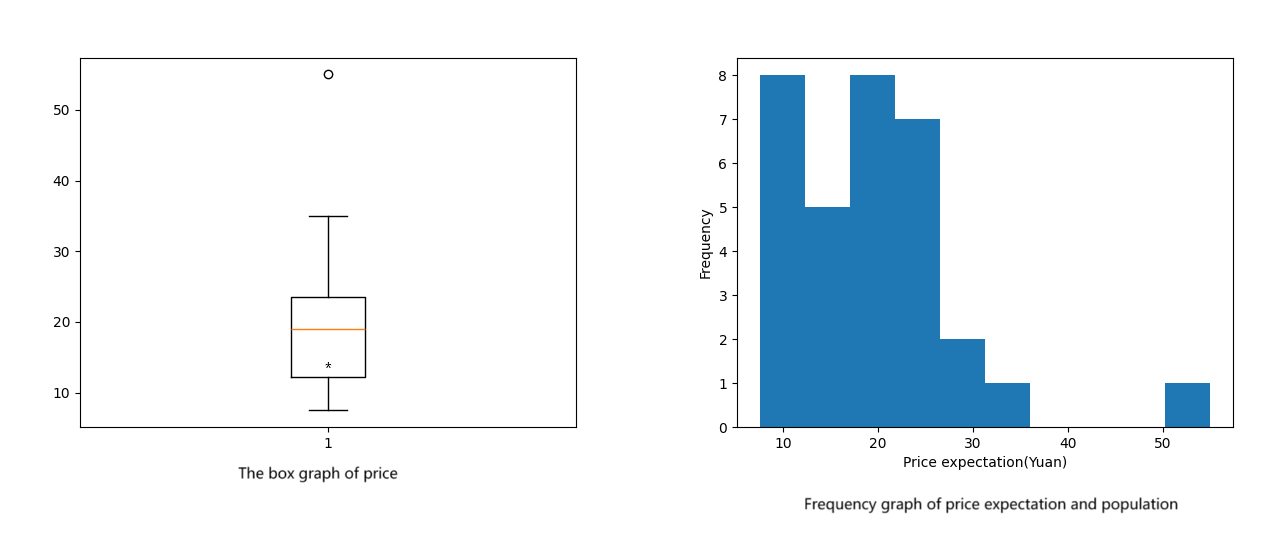
\includegraphics[width = 0.8\textwidth]{boxandhist.png}
    \caption{Price expectation}
    \label{fig.bnw} 
\end{figure}

In our survey, we first studied the price expectation of customers. Out of our $274$ questionnaires, only $32$ people volunteered to provide a reasonable price expectation of a 500ml cup of coffee. We tried to conduct one variable analysis on the collected data. The processing code is provided in appendix. As is shown in Figure \ref{fig.bnw}, there's one outlier among all data, which is a reasonable amount. If the outlier is excluded, we can find data in Table \ref{tab.onevar}.

\begin{center}
    \begin{threeparttable}[b]
        \centering
        %\begin{table}[h]
        \caption{Mean, std. deviation and five number summary}
        \label{tab.onevar}
        \begin{tabular}{llllllllll}
            \hline
            \textbf{Name}  & Sample size & Mean*    & Mean     & $\sigma$ \^{} & $\sigma^2$ (variance) & Range & \\ \hline
            \textbf{Value} & 32 & 19.28593 & 18.13387 & 6.93969 & 48.1596 &  27.5 & \\ \hline
            \textbf{Name} & Min. & Max. & IQR & Q1 & Q2(median) & Q3 \\ \hline
            \textbf{Value} & 7.5  & 35   & 18  & 13   & 23           & 31   \\ \hline
    
        \end{tabular}
        \begin{tablenotes}
        \footnotesize
        \item[*] Not excluding the outlier.
        \item[\^{}] Standard deviation.
        \end{tablenotes}
        %\end{table}
    \end{threeparttable}
    
\end{center}

In this chart, the mean ($\mu$), variation ($\sigma^2$), standard deviation ($\sigma$), interquartile range (IQR), range are given by the formulae:

\begin{equation*}
    \begin{aligned}
        \mu &= {{\sum_{i=1}^n a_i}\over n} \\
        \sigma^2 &= {{\sum_{i=1}^n (a_i-\mu)^2}\over n} \\
        \sigma &= \sqrt{\sigma^2}  \\
        \text{IQR} &= Q_3 - Q_1 \\
        \text{Range} &= \max\{a_i\} - \min\{a_i\} \\
    \end{aligned}
\end{equation*}

where $a_i$ refers to the $i$-th number of the data, $n$ is the size of the sample space, and $Q_1$ and $Q_3$ are the quartiles respectively.

The average price of a cup of Cotti coffee is $14$ yuan (denoted by a small asterisk mark in Figure \ref{fig.bnw}), located in the lower 25\%-50\% quartile. This means that Cotti coffee is a relatively affordable brand. 



\section{Two variable analysis}

As is shown in Figure \ref{fig.dc}, we plotted the price against the quantity by economics convention. This graph shows a significant negative correlation between $P$, the price, and $Q$, the quantity sold. This can be confirmed by a correlation coefficient of $-0.93828826$, which is close enough to $-1$ to show a strong negetive correlation. This coefficient is reasonable because customers are less likely to purchase a product when the price go up. However, there is still a point that does not follow this rule. It might because people do not think carefully when it comes to ``50\% off'' and ``-10 yuan'', where latter is a greater discount but the former sounds more attractive. This reminds managers of the importance of a well-organised advertising strategy.

Also, we found a linear fit of $y = -0.1331 x + 27.13$, where $x$ is the quantity demand and $y$ is the price. This equation fits well when $y$ does not deviate much, and the gradient means if the price goes up by $0.1331$ yuan, Cotti is likely to lose one customer. However, the y-intercept of $27.13$ yuan, which indicates if the price is higher than or equals to $27.13$ yuan, no one will be willing to purchase this product, is not reasonable. This means the linear fit model does not apply anymore when $y$ is siginificantly bigger than the current value.

\begin{figure}
    \centering
    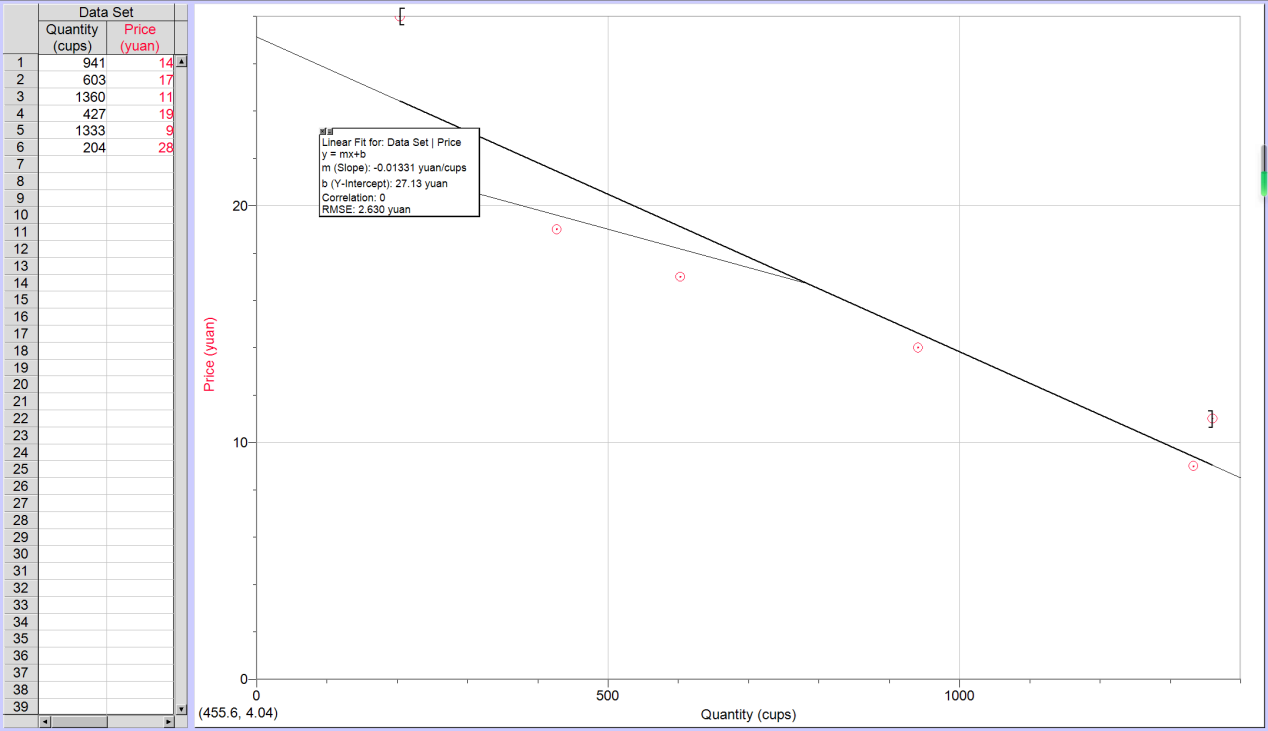
\includegraphics[width = 0.8\textwidth]{dc.png}
    \caption{Demand curve according to the data we collected}
    \label{fig.dc}
\end{figure}

%\textbf{Suggestions:}

\section{Contributions}

Our work distribution is listed here. Members are listed in alphabetical order.

\begin{itemize}
    \item Christie Chen Haonan: PPT making, evaluation of age distribution, 1/8 of math part.
    \item Elijah Dong Yicheng (group leader): PPT design and spread of questionnaires. Time management.
    \item Eric Zhou Changhui: Formatting, coding(calculation of PED), 3/4 of the math part.
    \item Kyle Dong Zeguang: Summary, spread of questionnaires, PPT design, photo taking, economics evaluation of portion of income.
    \item Warren Wang Yuanhao: Design of question paper, spread of question paper, introduction, 1/8 of math part.
\end{itemize}

\clearpage

\section*{Appendix}

\linespread{1}

\begin{lstlisting}[style = Python, caption={One variable analysis code}, label= code.1]
import matplotlib.pyplot as plt
import numpy as np
data = [55, 17.5, 27.5, 21.05, 25, 25, 10, 13, 30, 20, 9.9, 15, 15, 9.9, 18, 20, 8, 7.5, 25, 23, 23, 25, 21, 10, 35, 20, 18, 15, 22, 9.9, 9.9, 13]
plt.boxplot(data)
plt.show()
print(f"""mean:{sum(data)/len(data)},
          mean excluding outlier:{sum(data[1:])/len(data[1:])}
          min excl.{min(data[1:])}
          max excl.{max(data[1:])}
          std excl.{np.std(data[1:])}
          median {np.median(data[1:])}""")
data = sorted(data[1:])
print(data[int(len(data)/4)+1],data[int(3*len(data)/4)], len(data))
\end{lstlisting}

\begin{lstlisting}[style = Python, caption={Two variable analysis code}, label = code.2]
import numpy as np
data = """
941 14
603 17
1360    11
427 19
1333 9
204 28
""".split()
x, y = [], []
for dx in data:
    if len(x) == len(y): y += [int(dx)]
    else: x += [int(dx)]
xy = [(x[i], y[i]) for i in range(len(x))]
xy.sort(key = lambda t:  t[0])
x,y = ([xyi[z] for xyi in xy] for z in [0,1])
ped = []
print("x and y are respectively",x,y)
print("Their correlation coefficient is", np.corrcoef(x,y=y)[0][1])
for i in range(len(x)-1):
    dx = (x[i+1] - x[i]) / x[i]
    dy = (y[i+1] - y[i]) / y[i]
    ped += [dy/dx]
print("PED of the data is", ped)
\end{lstlisting}



% The sample size is too small to analyze on the histogram. The trend is not so clear.


\end{document}